\documentclass[12pt,a4paper,polish]{article}
\topmargin -1.6cm
\addtolength{\textheight}{4cm}
\textwidth  15.5cm

\leftmargin      5mm
\rightmargin     5mm
\oddsidemargin   5mm
\evensidemargin  5mm

\usepackage{hyperref}
\usepackage{polski}
\usepackage[utf8]{inputenc}
\usepackage{graphicx} % To jest pakiet do grafiki.
                      % Moze przydac sie pozniej.
\usepackage{units}
\usepackage{sty/wds}


\wdsTytulProjektu{Mój wspaniały projekt}
\wdsAutor{Jan Kowalski, 000007}




\begin{document}
%
% To po to, aby mieć format A4.
% pdflatex domyślnie tworzy dokument w formacie letter.
%
\pdfpageheight   297mm
\pdfpagewidth    210mm

\wdsStronaTytulowa
\wdsSpisTresci


 \section{Charakterystyka tematu projektu}
 \label{sekcja-charakterystyka}

  Opis projektu, podstawowe cele jakie ma pełnić dane
  urządzenie lub aplikacja, zasygnalizowanie podstawowych
  zagadnień związanych z danym tematem.

 \section{Podcele i etapy realizacji projektu}

  Bardziej szczegółowe przedstawienie zagadnień związanych
  z danym tematem. Wyodrębnienie podcelów.\\
  Lista podcelów:
  \begin{itemize}
    \item Przegląd literatury i zasobów Internetu związanych
          z tematem projektu
    \item Projekt układu elektronicznego (schemat ideowy)
    \item itd.
  \end{itemize}

 \section{Specyfikacja finalnego produktu}

  Jakie są spodziewane efekty realizowanego projektu.
  Jakie są oczekiwane zakresy mierzonych wartości, dokładności itp.

  
  \section{Terminarz realizacji poszczególnych podcelów 
                {\small (z dokładnością do 1 tygodnia)}}

  \begin{itemize}
    \item 21 marca 2022  -- zakończenie przeglądu materiałów
                            związanych z danym tematem
    \item 28 marca 2022 -- schemat układu elektronicznego
    \item  4 kwietnia 2022 -- $\ldots$
    \item 11 kwietnia 2022 -- $\ldots$
    \item 25 kwietnia 2022 -- $\ldots$
    \item  2 maja 2022 -- $\ldots$
    \item  9 maja 2022 -- $\ldots$
    \item 16 maja 2022 -- $\ldots$
    \item 23 maja 2022 -- $\ldots$
    \item 30 maja 2022 -- $\ldots$
    \item  6 czerwca 2022 -- $\ldots$
    \item 13 czerwca 2022 -- $\ldots$
    \item 20 czerwca 2022 -- $\ldots$
  \end{itemize}
  %
  Dopełnieniem harmonogramu powinien być diagram Gantta.




\section{{\it Kilka przykładów wykorzystania \LaTeX a} }

 To rozdział jest tu tylko po to, aby zaprezentować wybrane
 możliwości \LaTeX a.
 Przy odwoływaniu się do rozdziałów zawsze stosujemy odwołanie
 przez etykietę. Nigdy nie odwołujemy się wpisując konkretny
 numer, np. tutaj wykorzystując polecenie {\tt $\backslash$ref}
 można odwołać się do rozdziału \ref{sekcja-charakterystyka}.
 Można też podać stronę, na której ten rozdział jest, 
 np. patrz rodziła  \ref{sekcja-charakterystyka} 
(str.  \pageref{sekcja-charakterystyka}).
 Przy małych dokumentach to nie ma sensu, ale może się przydać
 przy większych.

 W ten sam sposób odwołujemy się do równań i wzorów,
 \begin{equation}
    F = ma
  \label{wzor-Newton2}
 \end{equation}
 np. możemy wskazać równianie (\ref{wzor-Newton2}).
 \begin{figure}[hbpt]
   \center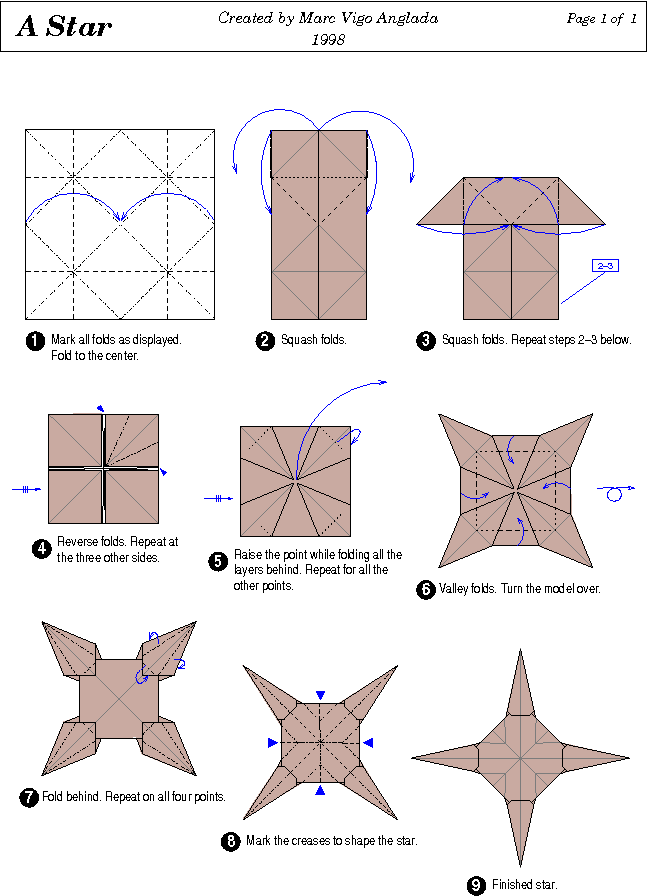
\includegraphics[width=6cm]{img/origami-gwiazda.png}
   \caption{Podpis pod rysunkiem.}
   \label{rysunek-gwiazda}
 \end{figure}
 W analogiczny sposób odwołujemy się do rysunków, tak
 jak np. do rys. \ref{rysunek-gwiazda} (Uwaga: etykieta musi
 być zdefiniowana po instrukcji {\tt $\backslash$caption}).\\[2ex]

 \noindent
     {\bf Uwaga: Do każdego rysunku, do każdej tabeli, jak też do każdego
          numerowanego równania musi być odwołanie w tekście.
 }\\[2ex]

 \noindent
 Literaturę należy cytować dowołując się do pozycji 
 z bazy bibliograficznej (jest ona w podkartotece {\tt bib}
 w pliku {\tt  baza\_bibliografii.bib}.
 Odwołujemy się również do nich również poprzez etykiety
 np. \cite{HTTP2}\cite{Hallam:PHD-thesis}
 lub \cite{Blanchette:Qt}. Etykietą jest
 pierwszy element w danej pozycji bibliograficznej.


\section{Przykłady zapisu jednostek z wykorzystaniem pakietu {\sf units}}

Opis pakietu: {\tt https://ctan.org/pkg/units}\\[1ex]
\begin{tabular}{rcl}
  Odległość/długość & -- & \unit[2,4]{m}             \\[1ex]
  Szybkość          & -- & \unitfrac[48]{km}{h}      \\[1ex]
  Szybkość          & -- & \unit[48]{$\frac{km}{h}$} \\[1ex]
  Napięcie          & -- & \unit[$-5$]{V}, \unit[$+12$]{V} \\[1ex]
  Kąt               & -- & 15$^\circ$
\end{tabular} 


\section{Łącznik, półpauza, myślnik, minus}

\LaTeX pozwala wygenerować trzy typy poziomych kreseczek i jedną specyficzną
dla trybu matematycznego oznaczającą znak minusa. Ich znaczenie opisane jest krótko poniżej.

\begin{itemize}
 \item[-]  $\leftarrow$ Ta krótka kreseczka oznacza łącznik i używana jest, tak jak jej nazwa
  wskazuje do łączenia wyrazów dla określenia odrębnej cechy lub obiektu, który
  opisywany jest tymi wyrazami, np. {\em flaga biało-czerwona.}

\item[--] $\leftarrow$ To jest półpauza. Wykorzystywana jest
  do oznaczania zakresu wartości, stron itd. np. {\em strony 12--16}.
  W polskim piśmiennictwie półpauzę wykorzystuje się jako myślnik,
  np.
  {\em Drużyna z Nowego Jorku – mająca doskonały zeszły sezon – grała poniżej oczekiwań.}

\item[---] $\leftarrow$ Jest to pauza. Wykorzystywana jest jako myślnik.
  Jednak tak jak zostało to wyżej napisane, w polskim piśmiennictwie raczej wykorzystuje się
  do tego celu półpauzę. Nie jest jednak błędem używanie pauzy. Należy jednak być wówczas
  konsekwentnym i stosować jako myślnik w całym tekście.
  Ten dłuższy myślnik jest charakterystyczne dla anglosaskiej
  typografii. Jednak należy pamiętać, że zapis zdania z myślnikiem w tekstach anglosaskich jest też inny.
  Nie może go poprzedzać spacja, jak też nie może być żadnej spacji za nim, np.\\
  {\em Mr.~Drofnats---or ``R. J.,'' as he preferred to be called---was happiest when he was at work.}

\item[$-$]  $\leftarrow$ To jest znak minus. Liczby ze znakiem należy zawsze zapisywać
  w trybie matematycznym, np. $+3$, $-12$.
\end{itemize}



\bibliographystyle{plplain}
\bibliography{baza_bibliografii}
\end{document}

